\documentclass[border=4pt]{standalone}

\usepackage[T1]{fontenc}
\usepackage[utf8]{inputenc}
\usepackage{amsmath}
\usepackage{xcolor}
\usepackage{tikz}
\usetikzlibrary{positioning, fit, calc, arrows.meta, backgrounds}

\begin{document}

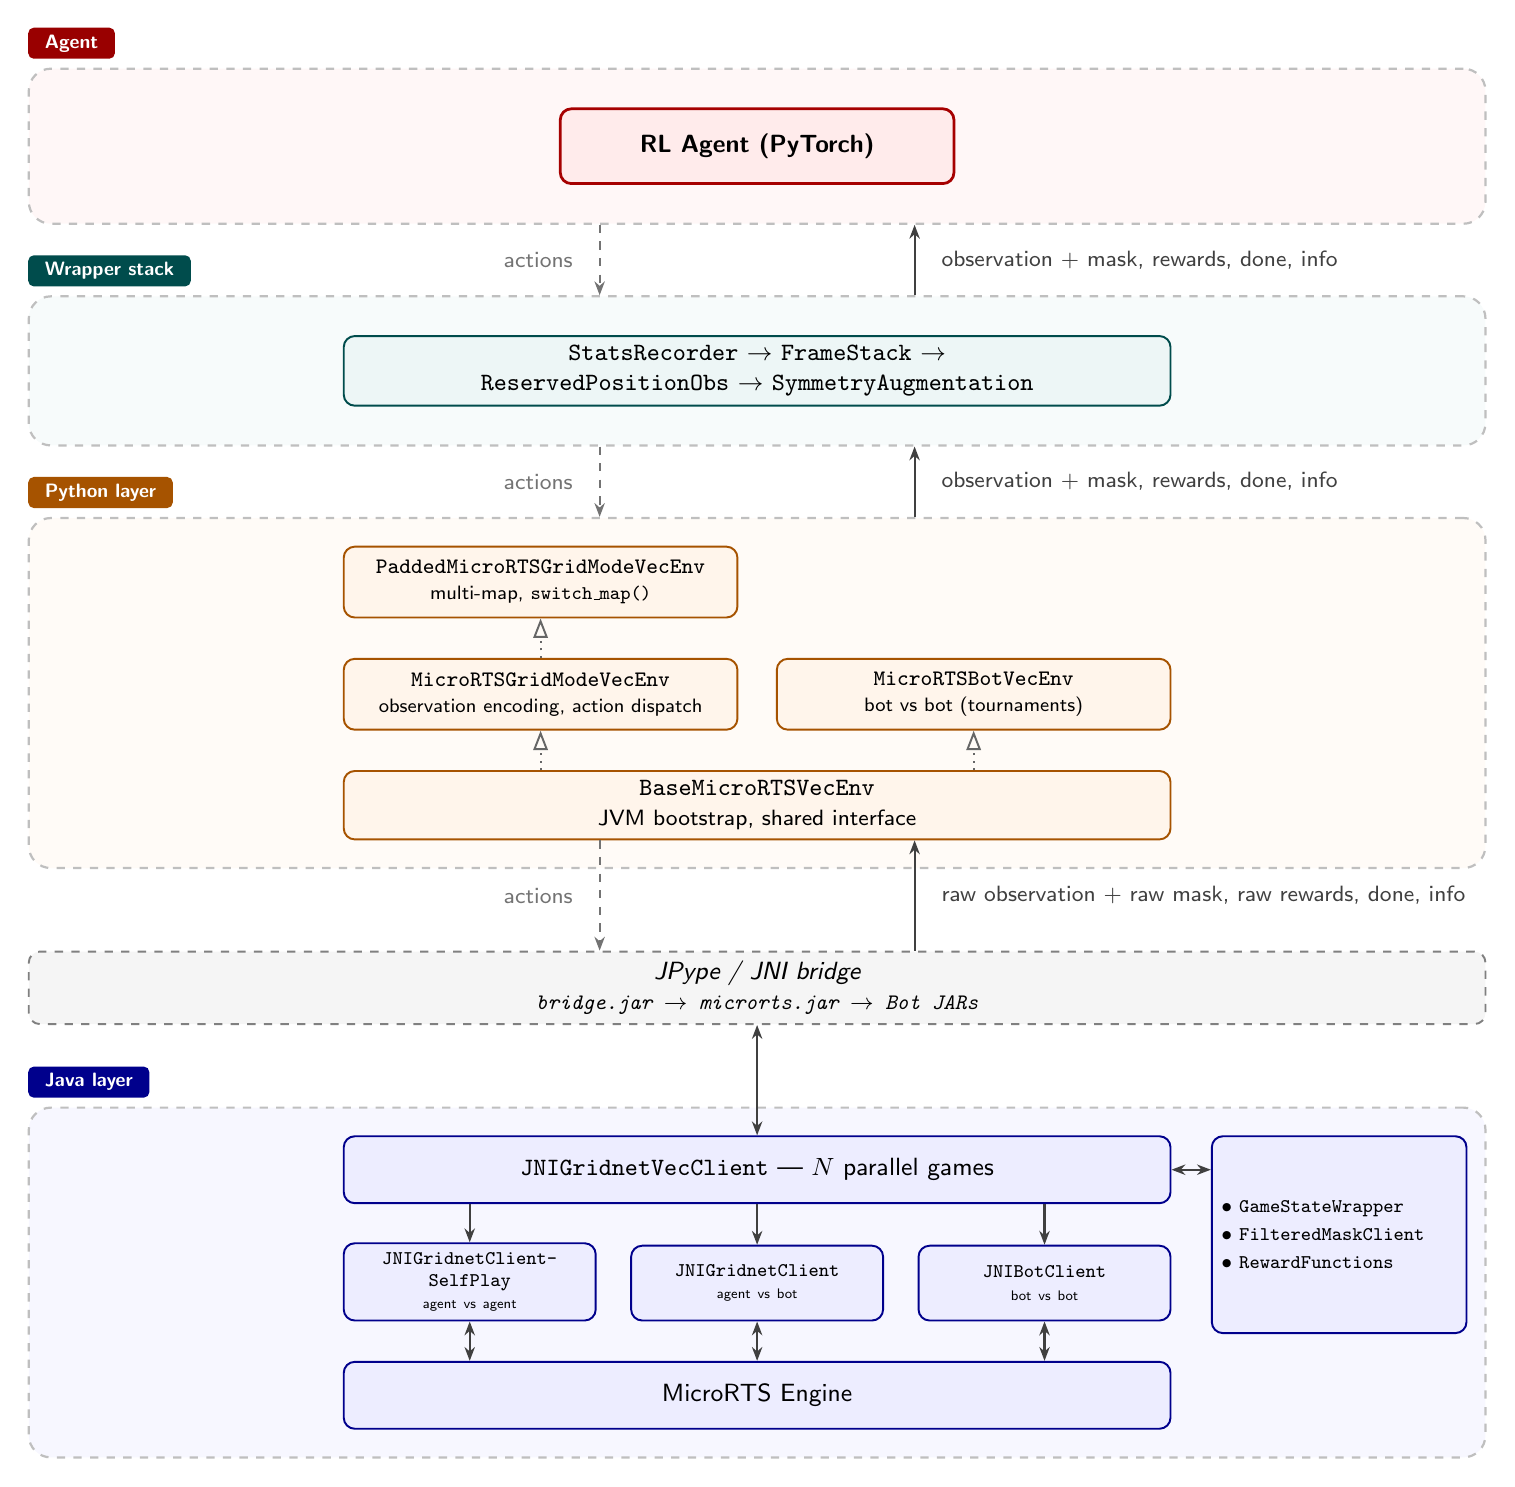
\begin{tikzpicture}[
    node distance=0.6cm,
    %% ── Palette ──
    javabox/.style={
        draw=blue!55!black, line width=0.7pt,
        rounded corners=4pt, fill=blue!7,
        minimum height=0.85cm, align=center, font=\small\sffamily},
    pybox/.style={
        draw=orange!65!black, line width=0.7pt,
        rounded corners=4pt, fill=orange!8,
        minimum height=0.85cm, align=center, font=\small\sffamily},
    wrapstyle/.style={
        draw=teal!60!black, line width=0.7pt,
        rounded corners=4pt, fill=teal!7,
        minimum height=0.75cm, align=center, font=\small\sffamily},
    agentstyle/.style={
        draw=red!65!black, line width=1pt,
        rounded corners=4pt, fill=red!8,
        minimum height=0.95cm, align=center, font=\small\bfseries\sffamily},
    bridgestyle/.style={
        draw=black!50, line width=0.7pt, dashed,
        rounded corners=4pt, fill=black!4,
        minimum height=0.8cm, align=center, font=\small\sffamily\itshape},
    subclient/.style={
        javabox, minimum width=3.2cm, text width=2.8cm,
        minimum height=0.95cm, font=\scriptsize\sffamily},
    envvar/.style={
        pybox, minimum width=5.0cm, minimum height=0.9cm,
        font=\footnotesize\sffamily},
    utilbox/.style={
        draw=blue!55!black, line width=0.7pt,
        rounded corners=4pt, fill=blue!7,
        align=left, font=\scriptsize\sffamily, text width=3.0cm},
    badge/.style={
        font=\scriptsize\sffamily\bfseries, text=white,
        rounded corners=2pt, inner xsep=6pt, inner ysep=2.5pt},
    fwd/.style={-{Stealth[length=5pt]}, line width=0.8pt, color=black!75},
    bwd/.style={-{Stealth[length=5pt]}, line width=0.8pt, dashed, color=black!55},
    bidir/.style={{Stealth[length=5pt]}-{Stealth[length=5pt]}, line width=0.8pt, color=black!75},
    inherit/.style={-{Triangle[open, length=7pt]}, line width=0.7pt, dotted, color=black!60},
    grp/.style={
        draw=black!25, line width=0.8pt, rounded corners=8pt,
        dashed, inner sep=10pt},
]

\def\BW{10.5cm}
\def\GW{18.5cm}

% ====================================================================
%  JAVA LAYER
% ====================================================================

\node[javabox, minimum width=\BW] (engine)
    {MicroRTS Engine};

\node[subclient, anchor=south west]
    at ([yshift=0.5cm]engine.north west) (selfplay)
    {\texttt{JNIGridnetClient\-SelfPlay}\\{\tiny agent vs agent}};

\node[subclient, anchor=south]
    at ([yshift=0.5cm]engine.north) (gridclient)
    {\texttt{JNIGridnetClient}\\{\tiny agent vs bot}};

\node[subclient, anchor=south east]
    at ([yshift=0.5cm]engine.north east) (botclient)
    {\texttt{JNIBotClient}\\{\tiny bot vs bot}};

\path (selfplay.north) -- (botclient.north) coordinate[midway] (sc_mid);
\node[javabox, minimum width=\BW, above=0.5cm of sc_mid] (vecclient)
    {\texttt{JNIGridnetVecClient} --- $N$ parallel games};

\node[utilbox, anchor=north west, minimum height=2.5cm] (javutils)
    at ([xshift=0.5cm]vecclient.north east)
    {$\bullet$~\texttt{GameStateWrapper}\\[2pt]
     $\bullet$~\texttt{FilteredMaskClient}\\[2pt]
     $\bullet$~\texttt{RewardFunctions}};

\begin{scope}[on background layer]
    \node[grp, fill=blue!3,
          fit=(engine)(selfplay)(botclient)(vecclient),
          minimum width=\GW] (javagroup) {};
\end{scope}
\node[badge, fill=blue!55!black, anchor=south west]
    at ([yshift=3pt]javagroup.north west) {Java layer};

\draw[fwd] (vecclient.south -| selfplay)   -- (selfplay.north);
\draw[fwd] (vecclient.south -| gridclient) -- (gridclient.north);
\draw[fwd] (vecclient.south -| botclient)  -- (botclient.north);
\draw[bidir] (selfplay.south)   -- (engine.north -| selfplay);
\draw[bidir] (gridclient.south) -- (engine.north -| gridclient);
\draw[bidir] (botclient.south)  -- (engine.north -| botclient);
\draw[bidir] (vecclient.east) -- (javutils.west |- vecclient.east);

% ====================================================================
%  JNI BRIDGE
% ====================================================================

\node[bridgestyle, minimum width=\GW, above=1.4cm of vecclient] (bridge)
    {\textit{JPype / JNI bridge}\\
     {\footnotesize\ttfamily bridge.jar $\to$ microrts.jar $\to$ Bot JARs}};

\draw[bidir] (vecclient.north) -- (bridge.south);

% ====================================================================
%  PYTHON LAYER
% ====================================================================

\node[pybox, minimum width=\BW, minimum height=0.85cm,
    above=1.4cm of bridge] (baseenv)
    {\texttt{BaseMicroRTSVecEnv}\\
     {\footnotesize JVM bootstrap, shared interface}};

\node[envvar, anchor=south west]
    at ([yshift=0.5cm]baseenv.north west) (gridenv)
    {\texttt{MicroRTSGridModeVecEnv}\\{\scriptsize observation encoding, action dispatch}};

\node[envvar, anchor=south east]
    at ([yshift=0.5cm]baseenv.north east) (botenv)
    {\texttt{MicroRTSBotVecEnv}\\{\scriptsize bot vs bot (tournaments)}};

\node[envvar, above=0.5cm of gridenv] (paddedenv)
    {\texttt{PaddedMicroRTSGridModeVecEnv}\\{\scriptsize multi-map, \texttt{switch\_map()}}};

\draw[inherit] (baseenv.north -| gridenv) -- (gridenv.south);
\draw[inherit] (baseenv.north -| botenv)  -- (botenv.south);
\draw[inherit] (gridenv.north) -- (paddedenv.south);

\begin{scope}[on background layer]
    \node[grp, fill=orange!3,
          fit=(baseenv)(gridenv)(botenv)(paddedenv),
          minimum width=\GW] (pygroup) {};
\end{scope}
\node[badge, fill=orange!65!black, anchor=south west]
    at ([yshift=3pt]pygroup.north west) {Python layer};

% ====================================================================
%  WRAPPER STACK
% ====================================================================

\node[wrapstyle, minimum width=\BW, above=1.4cm of pygroup.north] (wstack)
    {\texttt{StatsRecorder} $\to$ \texttt{FrameStack} $\to$ \\
     \texttt{ReservedPositionObs} $\to$ \texttt{SymmetryAugmentation}};

\begin{scope}[on background layer]
    \node[grp, fill=teal!3,
          fit=(wstack), inner ysep=14pt,
          minimum width=\GW] (wrapgroup) {};
\end{scope}
\node[badge, fill=teal!60!black, anchor=south west]
    at ([yshift=3pt]wrapgroup.north west) {Wrapper stack};

% ====================================================================
%  RL AGENT
% ====================================================================

\node[agentstyle, minimum width=5cm, above=1.4cm of wrapgroup.north] (agent)
    {RL Agent (PyTorch)};

\begin{scope}[on background layer]
    \node[grp, fill=red!3,
          fit=(agent), inner ysep=14pt, inner xsep=20pt,
          minimum width=\GW] (agentgroup) {};
\end{scope}
\node[badge, fill=red!60!black, anchor=south west]
    at ([yshift=3pt]agentgroup.north west) {Agent};

% ====================================================================
%  ARROWS — Bridge <-> Python
% ====================================================================

\draw[fwd] ([xshift=2cm]bridge.north)
    -- node[right, font=\footnotesize\sffamily, midway, xshift=6pt]
       {raw observation + raw mask, raw rewards, done, info}
    ([xshift=2cm]baseenv.south);

\draw[bwd] ([xshift=-2cm]baseenv.south)
    -- node[left, font=\footnotesize\sffamily, midway, xshift=-6pt]
       {actions}
    ([xshift=-2cm]bridge.north);

% ====================================================================
%  ARROWS — Python -> Wrappers
% ====================================================================

\draw[fwd] ([xshift=2cm]pygroup.north)
    -- node[right, font=\footnotesize\sffamily, midway, xshift=6pt]
       {observation + mask, rewards, done, info}
    ([xshift=2cm]wrapgroup.south);

\draw[bwd] ([xshift=-2cm]wrapgroup.south)
    -- node[left, font=\footnotesize\sffamily, midway, xshift=-6pt]
       {actions}
    ([xshift=-2cm]pygroup.north);

% ====================================================================
%  ARROWS — Wrappers <-> Agent
% ====================================================================

\draw[fwd] ([xshift=2cm]wrapgroup.north)
    -- node[right, font=\footnotesize\sffamily, midway, xshift=6pt]
       {observation + mask, rewards, done, info}
    ([xshift=2cm]agentgroup.south);

\draw[bwd] ([xshift=-2cm]agentgroup.south)
    -- node[left, font=\footnotesize\sffamily, midway, xshift=-6pt]
       {actions}
    ([xshift=-2cm]wrapgroup.north);

\end{tikzpicture}

\end{document}
